\begin{figure}[htb]
\centering
\includegraphics[page=6,width=0.25\textwidth]{\FCNCFigures/r21/thq2tau/SSOSWithFakeMCCalibrated/reg2mtau1b2jos/tautaumass.pdf}
\put(-30, 80){\textbf{(a1)}}
\includegraphics[page=6,width=0.25\textwidth]{\FCNCFigures/r21/thq2tau/SSOSWithFakeMCCalibrated/reg2mtau1b2jos/ttvismass.pdf}
\put(-30, 80){\textbf{(a2)}}
\includegraphics[page=6,width=0.25\textwidth]{\FCNCFigures/r21/thq2tau/SSOSWithFakeMCCalibrated/reg2mtau1b2jos/t1mass.pdf}
\put(-70, 70){\textbf{(a3)}}
\\
\includegraphics[page=6,width=0.25\textwidth]{\FCNCFigures/r21/thq2tau/SSOSWithFakeMCCalibrated/reg2mtau1b3jos/tautaumass.pdf}
\put(-30, 80){\textbf{(b1)}}
\includegraphics[page=6,width=0.25\textwidth]{\FCNCFigures/r21/thq2tau/SSOSWithFakeMCCalibrated/reg2mtau1b3jos/ttvismass.pdf}
\put(-30, 80){\textbf{(b2)}}
\includegraphics[page=6,width=0.25\textwidth]{\FCNCFigures/r21/thq2tau/SSOSWithFakeMCCalibrated/reg2mtau1b3jos/drtautau.pdf}
\put(-70, 70){\textbf{(b3)}}
\\
\includegraphics[page=6,width=0.25\textwidth]{\FCNCFigures/tthML/showFake/faketau/postfit/NOMINAL/reg1l1tau1b2j_os/drtautau.pdf}
\put(-30, 80){\textbf{(c1)}}
\includegraphics[page=6,width=0.25\textwidth]{\FCNCFigures/tthML/showFake/faketau/postfit/NOMINAL/reg1l1tau1b2j_os/tau_pt_0.pdf}
\put(-30, 80){\textbf{(c2)}}
\includegraphics[page=6,width=0.25\textwidth]{\FCNCFigures/tthML/showFake/faketau/postfit/NOMINAL/reg1l1tau1b2j_os/ttvismass.pdf}
\put(-70, 70){\textbf{(c3)}}
\\
\includegraphics[page=6,width=0.25\textwidth]{\FCNCFigures/tthML/showFake/faketau/postfit/NOMINAL/reg1l1tau1b3j_os/ttvismass.pdf}
\put(-30, 80){\textbf{(d1)}}
\includegraphics[page=6,width=0.25\textwidth]{\FCNCFigures/tthML/showFake/faketau/postfit/NOMINAL/reg1l1tau1b3j_os/tau_pt_0.pdf}
\put(-30, 80){\textbf{(d2)}}
\includegraphics[page=6,width=0.25\textwidth]{\FCNCFigures/tthML/showFake/faketau/postfit/NOMINAL/reg1l1tau1b3j_os/drtautau.pdf}
\put(-70, 70){\textbf{(d3)}}
\\
\includegraphics[page=6,width=0.25\textwidth]{\FCNCFigures/tthML/showFake/faketau/postfit/NOMINAL/reg1l2tau1bnj_os/ttvismass.pdf}
\put(-30, 80){\textbf{(e1)}}
\includegraphics[page=6,width=0.25\textwidth]{\FCNCFigures/tthML/showFake/faketau/postfit/NOMINAL/reg1l2tau1bnj_os/drtautau.pdf}
\put(-30, 80){\textbf{(e2)}}
\includegraphics[page=6,width=0.25\textwidth]{\FCNCFigures/tthML/showFake/faketau/postfit/NOMINAL/reg1l2tau1bnj_os/t2vismass.pdf}
\put(-70, 70){\textbf{(e3)}}
\\
\caption{ The BDT input distributions for the background and merged signal in the STH $\thadhad$ (a1-3), TTH $\thadhad$ (b1-3), STH $\tlhad$ (c1-3), TTH $\tlhad$ (d1-3),  $l\thadhad$ (e1-3) channels. }% The Kolmogorov Test values for the training and testing BDT distributions are also indicated.
\label{fig:mva_input}
\end{figure}